% Chapter 8: Modern Extensions in Time Series Analysis
% ARFIMA, Machine Learning (Random Forest, LSTM)
% Bachelor Program, Bucharest University of Economic Studies

\documentclass[9pt, aspectratio=169, t]{beamer}

% Ensure content fits on slides
\setbeamersize{text margin left=8mm, text margin right=8mm}

%=============================================================================
% THEME AND STYLE CONFIGURATION
%=============================================================================
\usetheme{Madrid}
\usecolortheme{seahorse}

% IDA-Inspired Color Palette
\definecolor{MainBlue}{RGB}{26, 58, 110}
\definecolor{AccentBlue}{RGB}{42, 82, 140}
\definecolor{IDAred}{RGB}{220, 53, 69}
\definecolor{DarkGray}{RGB}{51, 51, 51}
\definecolor{MediumGray}{RGB}{128, 128, 128}
\definecolor{LightGray}{RGB}{248, 248, 248}
\definecolor{VeryLightGray}{RGB}{235, 235, 235}
\definecolor{Crimson}{RGB}{220, 53, 69}
\definecolor{Forest}{RGB}{46, 125, 50}
\definecolor{Amber}{RGB}{181, 133, 63}
\definecolor{Orange}{RGB}{230, 126, 34}

\setbeamercolor{palette primary}{bg=MainBlue, fg=white}
\setbeamercolor{palette secondary}{bg=MainBlue!85, fg=white}
\setbeamercolor{palette tertiary}{bg=MainBlue!70, fg=white}
\setbeamercolor{structure}{fg=MainBlue}
\setbeamercolor{title}{fg=MainBlue}
\setbeamercolor{frametitle}{fg=MainBlue, bg=white}
\setbeamercolor{block title}{bg=MainBlue, fg=white}
\setbeamercolor{block body}{bg=VeryLightGray, fg=DarkGray}
\setbeamercolor{block title alerted}{bg=Crimson, fg=white}
\setbeamercolor{block body alerted}{bg=Crimson!8, fg=DarkGray}
\setbeamercolor{block title example}{bg=Forest, fg=white}
\setbeamercolor{block body example}{bg=Forest!8, fg=DarkGray}
\setbeamercolor{item}{fg=MainBlue}

\setbeamertemplate{navigation symbols}{}

\setbeamertemplate{footline}{
    \leavevmode%
    \hbox{%
        \begin{beamercolorbox}[wd=.333333\paperwidth,ht=2.5ex,dp=1ex,center]{author in head/foot}%
            \usebeamerfont{author in head/foot}\insertshortauthor
        \end{beamercolorbox}%
        \begin{beamercolorbox}[wd=.333333\paperwidth,ht=2.5ex,dp=1ex,center]{title in head/foot}%
            \usebeamerfont{title in head/foot}\insertshorttitle
        \end{beamercolorbox}%
        \begin{beamercolorbox}[wd=.333333\paperwidth,ht=2.5ex,dp=1ex,right]{date in head/foot}%
            \usebeamerfont{date in head/foot}\insertshortdate{}\hspace*{2em}
            \insertframenumber{} / \inserttotalframenumber\hspace*{2ex}
        \end{beamercolorbox}}%
    \vskip0pt%
}

%=============================================================================
% PACKAGES
%=============================================================================
\usepackage[utf8]{inputenc}
\usepackage[T1]{fontenc}
\usepackage{amsmath, amssymb, amsthm}
\usepackage{mathtools}
\usepackage{bm}
\usepackage{tikz}
\usetikzlibrary{arrows.meta, positioning, shapes, calc}
\usepackage{booktabs}
\usepackage{multirow}
\usepackage{array}
\usepackage{graphicx}
\usepackage{hyperref}
\hypersetup{colorlinks=false, pdfborder={0 0 0}}
\graphicspath{{../logos/}{../charts/}}

%=============================================================================
% THEOREM ENVIRONMENTS
%=============================================================================
\theoremstyle{definition}
\setbeamertemplate{theorems}[numbered]
\newtheorem{defn}{Definition}
\newtheorem{thm}{Theorem}
\newtheorem{prop}{Proposition}

%=============================================================================
% CUSTOM COMMANDS
%=============================================================================
\newcommand{\E}{\mathbb{E}}
\newcommand{\Var}{\text{Var}}
\newcommand{\Cov}{\text{Cov}}
\newcommand{\Corr}{\text{Corr}}
\newcommand{\R}{\mathbb{R}}

%=============================================================================
% TITLE INFORMATION
%=============================================================================
\title[Chapter 8: Modern Extensions]{Chapter 8: Modern Extensions}
\subtitle{Bachelor Program, Faculty of Cybernetics, Statistics and Economic Informatics, Bucharest University of Economic Studies}
\author[Prof. Daniel Traian Pele, PhD]{Prof. Daniel Traian Pele, PhD\\[0.2cm]\footnotesize\texttt{danpele@ase.ro}}
\institute{Bucharest University of Economic Studies}
\date{Academic Year 2025--2026}

\begin{document}

%=============================================================================
% TITLE SLIDE
%=============================================================================
\begin{frame}[plain]
    \begin{tikzpicture}[remember picture, overlay]
        \fill[IDAred] (current page.north west) rectangle ([yshift=-0.15cm]current page.north east);
        \node[anchor=north west] at ([xshift=0.5cm, yshift=-0.3cm]current page.north west) {
            \href{https://www.ase.ro}{\includegraphics[height=1.1cm]{ase_logo.png}}
        };
        \node[anchor=north] at ([yshift=-0.3cm]current page.north) {
            \href{https://ai4efin.ase.ro}{\includegraphics[height=1.1cm]{ai4efin_logo.png}}
        };
        \node[anchor=north east] at ([xshift=-0.5cm, yshift=-0.3cm]current page.north east) {
            \href{https://www.digital-finance-msca.com}{\includegraphics[height=1.1cm]{msca_logo.png}}
        };
    \end{tikzpicture}
    \vfill
    \begin{center}
        {\Large\textcolor{MediumGray}{Time Series Analysis and Forecasting}}\\[0.3cm]
        {\Huge\textbf{\textcolor{MainBlue}{Chapter 8: Modern Extensions}}}\\[0.5cm]
        {\Large\textcolor{IDAred}{ARFIMA, Machine Learning, Deep Learning}}
    \end{center}
    \vfill

    \begin{tikzpicture}[remember picture, overlay]
        \fill[IDAred] (current page.south west) rectangle ([yshift=0.15cm]current page.south east);
        \node[anchor=south west] at ([xshift=0.5cm, yshift=0.8cm]current page.south west) {
            \href{https://theida.net}{\includegraphics[height=0.9cm]{ida_logo.png}}
        };
        \node[anchor=south] at ([xshift=-3cm, yshift=0.8cm]current page.south) {
            \href{https://blockchain-research-center.com}{\includegraphics[height=0.9cm]{brc_logo.png}}
        };
        \node[anchor=south] at ([yshift=0.8cm]current page.south) {
            \href{https://quantinar.com}{\includegraphics[height=0.9cm]{qr_logo.png}}
        };
        \node[anchor=south] at ([xshift=3cm, yshift=0.8cm]current page.south) {
            \href{https://quantlet.com}{\includegraphics[height=0.9cm]{ql_logo.png}}
        };
        \node[anchor=south east] at ([xshift=-0.5cm, yshift=0.8cm]current page.south east) {
            \href{https://ipe.ro/new}{\includegraphics[height=0.9cm]{acad_logo.png}}
        };
    \end{tikzpicture}
\end{frame}

%=============================================================================
% OUTLINE
%=============================================================================
\begin{frame}{Contents}
    \vspace{-0.5cm}
    {\scriptsize
    \begin{columns}[T]
        \begin{column}{0.32\textwidth}
            \tableofcontents[sections={1-4}, hideallsubsections]
        \end{column}
        \begin{column}{0.32\textwidth}
            \tableofcontents[sections={5-7}, hideallsubsections]
        \end{column}
        \begin{column}{0.32\textwidth}
            \tableofcontents[sections={8-10}, hideallsubsections]
        \end{column}
    \end{columns}
    }
\end{frame}

%=============================================================================
% LEARNING OBJECTIVES
%=============================================================================
\begin{frame}{Learning Objectives}
    \begin{block}{By the end of this chapter, you will be able to:}
        \begin{enumerate}
            \item Understand the concept of \textbf{long memory} in time series
            \item Estimate and interpret \textbf{ARFIMA}
            \item Apply \textbf{Random Forest} for time series forecasting
            \item Build \textbf{LSTM} networks for time series
            \item Compare performance of classical vs ML models
            \item Choose the appropriate method based on context
            \item Implement these methods in \textbf{Python}
        \end{enumerate}
    \end{block}
\end{frame}

%=============================================================================
\section{Motivation}
%=============================================================================

\begin{frame}{From Classical Models to Machine Learning}
    \begin{block}{Limitations of ARIMA Models}
        \begin{itemize}
            \item Assume \textbf{short memory}: autocorrelations decay exponentially
            \item Relationships \textbf{linear} between variables
            \item Difficulties with \textbf{complex patterns} and nonlinear
            \item Requires \textbf{stationarity} (through differencing)
        \end{itemize}
    \end{block}

    \vspace{0.2cm}

    \begin{alertblock}{Modern Solutions}
        \begin{itemize}
            \item \textbf{ARFIMA}: Captures long memory (autocorrelations that decay slowly)
            \item \textbf{Random Forest}: Nonlinear relationships, robust to outliers
            \item \textbf{LSTM}: Complex sequential patterns, long-term dependencies
        \end{itemize}
    \end{alertblock}
\end{frame}

\begin{frame}{When to Use Each Method?}
    \begin{center}
    \begin{tabular}{l|c|c|c|c}
        \toprule
        \textbf{Feature} & \textbf{ARIMA} & \textbf{ARFIMA} & \textbf{RF} & \textbf{LSTM} \\
        \midrule
        Long memory & $\times$ & $\checkmark$ & $\checkmark$ & $\checkmark$ \\
        Relationships nonlinear & $\times$ & $\times$ & $\checkmark$ & $\checkmark$ \\
        Interpretability & $\checkmark$ & $\checkmark$ & $\sim$ & $\times$ \\
        Few data & $\checkmark$ & $\checkmark$ & $\times$ & $\times$ \\
        Exogenous variables & $\checkmark$ & $\checkmark$ & $\checkmark$ & $\checkmark$ \\
        Uncertainty & $\checkmark$ & $\checkmark$ & $\sim$ & $\times$ \\
        \bottomrule
    \end{tabular}
    \end{center}

    \vspace{0.3cm}

    \begin{exampleblock}{Golden Rule}
        Start \textbf{simple} (ARIMA), then increase complexity only if justified by data and performance.
    \end{exampleblock}
\end{frame}

%=============================================================================
\section{ARFIMA: Modele cu Long Memory}
%=============================================================================

\begin{frame}{What is Long Memory?}
    \begin{block}{Short Memory (ARMA)}
        \begin{itemize}
            \item Autocorrelations $\rho_k$ decay \textbf{exponentially}: $|\rho_k| \leq C \cdot r^k$, $r < 1$
            \item Shock effects disappear \textbf{quickly}
            \item Finite sum: $\sum_{k=0}^{\infty} |\rho_k| < \infty$
        \end{itemize}
    \end{block}

    \vspace{0.2cm}

    \begin{alertblock}{Long Memory (ARFIMA)}
        \begin{itemize}
            \item Autocorrelations decay \textbf{hyperbolically}: $\rho_k \sim C \cdot k^{2d-1}$
            \item Shock effects persist \textbf{for a long time}
            \item Infinite sum: $\sum_{k=0}^{\infty} |\rho_k| = \infty$ (for $d > 0$)
        \end{itemize}
    \end{alertblock}

    \vspace{0.2cm}

    \begin{exampleblock}{Exemple cu Long Memory}
        Financial market volatility, river flows, network traffic, inflation
    \end{exampleblock}
\end{frame}

\begin{frame}{Comparație ACF: Short Memory vs Lungă}
    \begin{center}
        \includegraphics[width=0.95\textwidth, height=0.75\textheight, keepaspectratio]{charts/ch8_acf_comparison.pdf}
    \end{center}
    \vspace{-0.3cm}
    {\footnotesize
    \textbf{Left}: AR(1) --- autocorrelations decay exponentially (short memory)\\
    \textbf{Right}: ARFIMA with $d=0.35$ --- autocorrelations decay hyperbolically (long memory)
    }
\end{frame}

\begin{frame}{The ARFIMA Model(p,d,q)}
    \begin{defn}[ARFIMA]
        A process $\{Y_t\}$ follows a \textbf{ARFIMA(p,d,q)} if:
        $$\phi(L)(1-L)^d Y_t = \theta(L)\varepsilon_t$$
        where $d \in (-0.5, 0.5)$ is the \textbf{fractional differencing parameter}.
    \end{defn}

    \vspace{0.3cm}

    \begin{block}{Fractional Differencing Operator}
        $$(1-L)^d = \sum_{k=0}^{\infty} \binom{d}{k}(-L)^k = 1 - dL - \frac{d(1-d)}{2!}L^2 - \frac{d(1-d)(2-d)}{3!}L^3 - \cdots$$
    \end{block}

    \vspace{0.2cm}

    {\small
    \begin{itemize}
        \item $d = 0$: ARMA standard (short memory)
        \item $0 < d < 0.5$: Long memory, stationarity
        \item $d = 0.5$: Stationarity limit
        \item $0.5 \leq d < 1$: Nestationarity, dar mean-reverting
        \item $d = 1$: Random walk (ARIMA standard)
    \end{itemize}
    }
\end{frame}

\begin{frame}{Interpreting the Parameter $d$}
    \begin{center}
    \begin{tabular}{c|l|l}
        \toprule
        \textbf{Value $d$} & \textbf{ACF Behavior} & \textbf{Interpretation} \\
        \midrule
        $d = 0$ & Scădere exponentiallyă & Memorie scurtă \\
        $0 < d < 0.5$ & Scădere hyperbolically & Long memory, stationary \\
        $d = 0.5$ & Non-summable ACF & At the limit \\
        $0.5 < d < 1$ & Very slow decay & Long memory, nestationary \\
        $d = 1$ & ACF = 1 (constant) & Random walk \\
        \bottomrule
    \end{tabular}
    \end{center}

    \vspace{0.3cm}

    \begin{block}{Hurst Parameter $H$}
        Relationship with Hurst exponent: $d = H - 0.5$
        \begin{itemize}
            \item $H = 0.5$: Random walk (no memory)
            \item $H > 0.5$: Persistence (trend-following)
            \item $H < 0.5$: Anti-persistence (mean-reverting)
        \end{itemize}
    \end{block}
\end{frame}

\begin{frame}{Effect of Parameter $d$ on ACF}
    \begin{center}
        \includegraphics[width=0.95\textwidth, height=0.75\textheight, keepaspectratio]{charts/ch8_arfima_d_effect.pdf}
    \end{center}
    \vspace{-0.2cm}
    {\footnotesize
    The higher $d$, the slower autocorrelations decay. As $d \to 0.5$, autocorrelations remain significant even at very large lags.
    }
\end{frame}

\begin{frame}{Exponentul Hurst: Interpretation Vizuală}
    \begin{center}
        \includegraphics[width=0.95\textwidth, height=0.70\textheight, keepaspectratio]{charts/ch8_hurst_interpretation.pdf}
    \end{center}
    \vspace{-0.2cm}
    {\footnotesize
    \textbf{H $<$ 0.5}: Series that frequently returns to mean (mean-reverting)\\
    \textbf{H = 0.5}: Random walk, unpredictable\\
    \textbf{H $>$ 0.5}: Persistent series, trends continue
    }
\end{frame}

\begin{frame}{Estimating the Parameter $d$}
    \begin{block}{Estimation Methods}
        \begin{enumerate}
            \item \textbf{GPH (Geweke-Porter-Hudak)}: Regression in frequency domain
            $$\ln I(\omega_j) = c - d \cdot \ln\left(4\sin^2\frac{\omega_j}{2}\right) + \varepsilon_j$$

            \item \textbf{R/S (Rescaled Range)}: Hurst method
            $$\frac{R}{S}(n) \sim c \cdot n^H$$

            \item \textbf{MLE (Maximum Likelihood)}: Full ARFIMA estimation

            \item \textbf{Whittle}: Efficient approximation in frequency domain
        \end{enumerate}
    \end{block}

    \vspace{0.2cm}

    {\footnotesize
    În Python: \texttt{arch} package, \texttt{statsmodels.tsa.arima.model.ARIMA} cu \texttt{order=(p,d,q)} where $d$ poate fi fractional.
    }
\end{frame}

\begin{frame}{ARFIMA Example in Python}
    \begin{block}{Python Code}
        {\footnotesize
        \texttt{from statsmodels.tsa.arima.model import ARIMA}

        \texttt{model = ARIMA(y, order=(1, 0.3, 1))}

        \texttt{results = model.fit()}
        }
    \end{block}

    \vspace{0.2cm}

    \begin{alertblock}{Note}
        ARFIMA estimation requires specialized packages. In practice, one often uses \texttt{arch} or \texttt{fracdiff} in Python.
    \end{alertblock}
\end{frame}

\begin{frame}{Exemplu Real: Long Memory în Volatility}
    \begin{center}
        \includegraphics[width=0.98\textwidth, height=0.72\textheight, keepaspectratio]{charts/ch8_volatility_long_memory.pdf}
    \end{center}
    \vspace{-0.3cm}
    {\footnotesize
    \textbf{Stylized Fact}: Financial returns have short memory, but volatility (|returns|) has long memory! This is the basis for FIGARCH models.
    }
\end{frame}

%=============================================================================
\section{Random Forest for Serii de Timp}
%=============================================================================

\begin{frame}{Random Forest: Basic Concepts}
    \begin{block}{What is Random Forest?}
        \begin{itemize}
            \item \textbf{Ensemble} of decision trees
            \item Each tree trained on a \textbf{bootstrap subset} of the data
            \item At each node, a \textbf{randomly} subset of features is selected
            \item Final prediction = \textbf{average} of all tree predictions
        \end{itemize}
    \end{block}

    \vspace{0.2cm}

    \begin{exampleblock}{Avantaje for Serii de Timp}
        \begin{itemize}
            \item Captures \textbf{nonlinear relationships}
            \item \textbf{Robust} to outliers and noise
            \item Does not require \textbf{stationarity}
            \item Provides \textbf{feature importance} (interpretability)
            \item Works well with \textbf{many variables}
        \end{itemize}
    \end{exampleblock}
\end{frame}

\begin{frame}{Pregătirea Yestelor for Random Forest}
    \begin{block}{Feature Engineering for Serii de Timp}
        \begin{enumerate}
            \item \textbf{Lag features}: $Y_{t-1}, Y_{t-2}, \ldots, Y_{t-p}$
            \item \textbf{Rolling statistics}: moving average, standard deviation
            \item \textbf{Calendar features}: day of week, month, season
            \item \textbf{Trend features}: time, quadratic trend
            \item \textbf{Exogenous variables}: economic indicators, events
        \end{enumerate}
    \end{block}

    \vspace{0.2cm}

    \begin{alertblock}{Warning: Data Leakage!}
        \begin{itemize}
            \item Do not use future information in features
            \item Train/test split: \textbf{temporal}, nu randomly!
            \item Rolling statistics: calculate only on \textbf{past data}
        \end{itemize}
    \end{alertblock}
\end{frame}

\begin{frame}{Feature Engineering: Illustration}
    \begin{center}
        \includegraphics[width=0.98\textwidth, height=0.75\textheight, keepaspectratio]{charts/ch8_feature_engineering.pdf}
    \end{center}
    \vspace{-0.3cm}
    {\footnotesize
    We transform the time series into features: lags, rolling statistics, and the RF model learns relationships between these and future values.
    }
\end{frame}

\begin{frame}{Random Forest: Python Implementation}
    \begin{block}{Python Code}
        {\footnotesize
        \texttt{from sklearn.ensemble import RandomForestRegressor}

        \texttt{rf = RandomForestRegressor(n\_estimators=100, max\_depth=10)}

        \texttt{rf.fit(X\_train, y\_train)}

        \texttt{predictions = rf.predict(X\_test)}
        }
    \end{block}
\end{frame}

\begin{frame}{Importanța Features and Interpretation}
    \begin{block}{Feature Importance}
        Random Forest provides importance measures:
        \begin{itemize}
            \item \textbf{Mean Decrease Impurity (MDI)}: Reduction in impurity at each split
            \item \textbf{Permutation Importance}: Cât decaye performanța când feature-ul e permutat randomly
        \end{itemize}
    \end{block}

    \vspace{0.2cm}

    \begin{exampleblock}{Interpretation Tipică for Serii de Timp}
        \begin{itemize}
            \item \texttt{lag\_1} very important $\Rightarrow$ Strong autocorrelation
            \item \texttt{rolling\_mean} important $\Rightarrow$ Local trend matters
            \item \texttt{month} important $\Rightarrow$ Seasonality present
        \end{itemize}
    \end{exampleblock}

    \vspace{0.2cm}

    {\footnotesize
    \texttt{rf.feature\_importances\_} or \texttt{permutation\_importance(rf, X\_test, y\_test)}
    }
\end{frame}

\begin{frame}{Random Forest: Forecast Example}
    \begin{center}
        \includegraphics[width=0.98\textwidth, height=0.72\textheight, keepaspectratio]{charts/ch8_rf_prediction.pdf}
    \end{center}
    \vspace{-0.3cm}
    {\footnotesize
    The Random Forest model trained on historical data (blue) produces forecasts (red dotted) that closely follow actual values in the test period (green).
    }
\end{frame}

%=============================================================================
\section{LSTM: Deep Learning for Serii de Timp}
%=============================================================================

\begin{frame}{Recurrent Neural Networks (RNN)}
    \begin{block}{Basic Idea}
        \begin{itemize}
            \item Networks that process \textbf{sequences} of data
            \item Have \textbf{internal memory} (hidden state)
            \item Current state depends on input + previous state
        \end{itemize}
    \end{block}

    \vspace{0.2cm}

    \begin{center}
    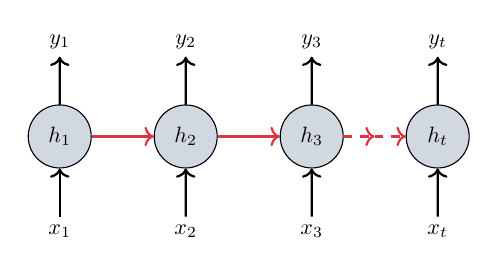
\begin{tikzpicture}[scale=0.8, transform shape]
        \node[draw, circle, minimum size=1cm, fill=MainBlue!20] (h1) at (0,0) {$h_1$};
        \node[draw, circle, minimum size=1cm, fill=MainBlue!20] (h2) at (2,0) {$h_2$};
        \node[draw, circle, minimum size=1cm, fill=MainBlue!20] (h3) at (4,0) {$h_3$};
        \node[draw, circle, minimum size=1cm, fill=MainBlue!20] (ht) at (6,0) {$h_t$};

        \node (x1) at (0,-1.5) {$x_1$};
        \node (x2) at (2,-1.5) {$x_2$};
        \node (x3) at (4,-1.5) {$x_3$};
        \node (xt) at (6,-1.5) {$x_t$};

        \node (y1) at (0,1.5) {$y_1$};
        \node (y2) at (2,1.5) {$y_2$};
        \node (y3) at (4,1.5) {$y_3$};
        \node (yt) at (6,1.5) {$y_t$};

        \draw[->, thick] (x1) -- (h1);
        \draw[->, thick] (x2) -- (h2);
        \draw[->, thick] (x3) -- (h3);
        \draw[->, thick] (xt) -- (ht);

        \draw[->, thick] (h1) -- (y1);
        \draw[->, thick] (h2) -- (y2);
        \draw[->, thick] (h3) -- (y3);
        \draw[->, thick] (ht) -- (yt);

        \draw[->, thick, IDAred] (h1) -- (h2);
        \draw[->, thick, IDAred] (h2) -- (h3);
        \draw[->, thick, IDAred, dashed] (h3) -- (5,0);
        \draw[->, thick, IDAred, dashed] (5,0) -- (ht);
    \end{tikzpicture}
    \end{center}

    \begin{alertblock}{Problem: Vanishing Gradient}
        Simple RNNs ``forget'' information from the distant past.
    \end{alertblock}
\end{frame}

\begin{frame}{LSTM: Long Short-Term Memory}
    \begin{block}{The LSTM Solution}
        Special cells with \textbf{3 gates} that control information flow:
        \begin{itemize}
            \item \textbf{Forget Gate} ($f_t$): Ce să forgetm din memoria anterioară
            \item \textbf{Input Gate} ($i_t$): What new information to add
            \item \textbf{Output Gate} ($o_t$): What to send to output
        \end{itemize}
    \end{block}

    \vspace{0.2cm}

    \begin{block}{LSTM Equations}
        {\small
        \begin{align*}
            f_t &= \sigma(W_f \cdot [h_{t-1}, x_t] + b_f) & \text{(Forget)} \\
            i_t &= \sigma(W_i \cdot [h_{t-1}, x_t] + b_i) & \text{(Input)} \\
            \tilde{C}_t &= \tanh(W_C \cdot [h_{t-1}, x_t] + b_C) & \text{(Candidate)} \\
            C_t &= f_t \odot C_{t-1} + i_t \odot \tilde{C}_t & \text{(Cell state)} \\
            o_t &= \sigma(W_o \cdot [h_{t-1}, x_t] + b_o) & \text{(Output)} \\
            h_t &= o_t \odot \tanh(C_t) & \text{(Hidden state)}
        \end{align*}
        }
    \end{block}
\end{frame}

\begin{frame}{LSTM Cell Architecture}
    \begin{center}
        \includegraphics[width=0.95\textwidth, height=0.75\textheight, keepaspectratio]{charts/ch8_lstm_architecture.pdf}
    \end{center}
    \vspace{-0.2cm}
    {\footnotesize
    Gates (forget, input, output) control what information is forgotten, added, and transmitted. \textbf{Cell state} allows gradients to ``flow'' without degradation.
    }
\end{frame}

\begin{frame}{Avantajele LSTM for Serii de Timp}
    \begin{exampleblock}{Why LSTM?}
        \begin{itemize}
            \item Captures \textbf{long-term dependencies} (spre deosebire de Simple RNNs)
            \item Learns \textbf{complex patterns} and nonlinear
            \item Handles \textbf{sequences de lungimi variabile}
            \item Works well with \textbf{multivariate data}
        \end{itemize}
    \end{exampleblock}

    \vspace{0.2cm}

    \begin{alertblock}{Disadvantages}
        \begin{itemize}
            \item Requires \textbf{lots of data} for training
            \item \textbf{Computationally intensive}
            \item ``\textbf{Black box}'' - hard to interpret
            \item Sensitive to \textbf{hyperparameters}
            \item Can \textbf{overfit} easily
        \end{itemize}
    \end{alertblock}
\end{frame}

\begin{frame}{LSTM: Implementare in Python cu Keras}
    \begin{block}{Python Code}
        {\footnotesize
        \texttt{from tensorflow.keras.models import Sequential}

        \texttt{from tensorflow.keras.layers import LSTM, Dense, Dropout}

        \vspace{0.2cm}
        \texttt{model = Sequential([}

        \texttt{~~~~LSTM(50, return\_sequences=True, input\_shape=(n, 1)),}

        \texttt{~~~~Dropout(0.2),}

        \texttt{~~~~LSTM(50),}

        \texttt{~~~~Dense(1)}

        \texttt{])}

        \texttt{model.compile(optimizer='adam', loss='mse')}
        }
    \end{block}
\end{frame}

\begin{frame}{Pregătirea Yestelor for LSTM}
    \begin{block}{Essential Steps}
        \begin{enumerate}
            \item \textbf{Normalization/Scaling}: MinMaxScaler or StandardScaler
            \item \textbf{Creare sequences}: Sliding window for input
            \item \textbf{Reshape}: 3D format (samples, timesteps, features)
            \item \textbf{Train/Test split}: Temporal, nu randomly!
        \end{enumerate}
    \end{block}

    \vspace{0.2cm}

    \begin{block}{Example Creating Sequences}
        {\footnotesize
        \texttt{def create\_sequences(data, n\_steps):}

        \texttt{~~~~X, y = [], []}

        \texttt{~~~~for i in range(len(data) - n\_steps):}

        \texttt{~~~~~~~~X.append(data[i:(i + n\_steps)])}

        \texttt{~~~~return np.array(X), np.array(y)}

        \vspace{0.1cm}
        \texttt{X, y = create\_sequences(scaled\_data, 10)}
        }
    \end{block}
\end{frame}

%=============================================================================
\section{Comparison and Model Selection}
%=============================================================================

\begin{frame}{Evaluation Metrics}
    \begin{block}{Common Metrics}
        \begin{itemize}
            \item \textbf{RMSE}: $\sqrt{\frac{1}{n}\sum_{i=1}^n (y_i - \hat{y}_i)^2}$ --- Error in original units
            \item \textbf{MAE}: $\frac{1}{n}\sum_{i=1}^n |y_i - \hat{y}_i|$ --- Robust to outliers
            \item \textbf{MAPE}: $\frac{100}{n}\sum_{i=1}^n \left|\frac{y_i - \hat{y}_i}{y_i}\right|$ --- Percentage error
            \item \textbf{MASE}: Compared to naive benchmark
        \end{itemize}
    \end{block}

    \vspace{0.2cm}

    \begin{alertblock}{Validare for Serii de Timp}
        \begin{itemize}
            \item \textbf{Do not} use standard cross-validation!
            \item Use \textbf{Time Series Cross-Validation} (walk-forward)
            \item Or \textbf{train/validation/test} temporal split
        \end{itemize}
    \end{alertblock}
\end{frame}

\begin{frame}{Time Series Cross-Validation}
    \begin{center}
        \includegraphics[width=0.95\textwidth, height=0.60\textheight, keepaspectratio]{charts/ch8_timeseries_cv.pdf}
    \end{center}

    \vspace{0.2cm}

    \begin{block}{Python Implementation}
        {\footnotesize
        \texttt{from sklearn.model\_selection import TimeSeriesSplit}

        \texttt{tscv = TimeSeriesSplit(n\_splits=5)}
        }
    \end{block}

    {\footnotesize
    \textbf{Important}: Setul de training crește progresiv, and test is always in the future. This way we avoid data leakage.
    }
\end{frame}

\begin{frame}{Model Selection Guide}
    {\small
    \begin{center}
    \begin{tikzpicture}[
        node distance=1.5cm,
        decision/.style={diamond, draw, fill=MainBlue!20, text width=2.5cm, align=center, inner sep=1pt},
        block/.style={rectangle, draw, fill=Forest!20, text width=2cm, align=center, rowhered corners},
        arrow/.style={thick,->,>=stealth}
    ]
        \node[decision] (start) {Few data?};
        \node[block, below left=1cm and 1.5cm of start] (arima) {ARIMA/ ARFIMA};
        \node[decision, below right=1cm and 1.5cm of start] (nonlin) {Relationships nonlinear?};
        \node[block, below left=1cm and 0.5cm of nonlin] (arfima) {ARFIMA};
        \node[decision, below right=1cm and 0.5cm of nonlin] (interp) {Interpretable?};
        \node[block, below left=0.8cm and 0cm of interp] (rf) {Random Forest};
        \node[block, below right=0.8cm and 0cm of interp] (lstm) {LSTM};

        \draw[arrow] (start) -- node[above left] {Yes} (arima);
        \draw[arrow] (start) -- node[above right] {Do not} (nonlin);
        \draw[arrow] (nonlin) -- node[above left] {Do not} (arfima);
        \draw[arrow] (nonlin) -- node[above right] {Yes} (interp);
        \draw[arrow] (interp) -- node[above left] {Yes} (rf);
        \draw[arrow] (interp) -- node[above right] {Do not} (lstm);
    \end{tikzpicture}
    \end{center}
    }
\end{frame}

\begin{frame}{Model Comparison: Accuracy vs Computational Cost}
    \begin{center}
        \includegraphics[width=0.98\textwidth, height=0.72\textheight, keepaspectratio]{charts/ch8_model_comparison.pdf}
    \end{center}
    \vspace{-0.3cm}
    {\footnotesize
    \textbf{Trade-off}: Modelele ML pot avea acuratețe easily mai bună, but computational cost increases significantly. Pentru few data or interpretability, ARIMA/ARFIMA remain excellent choices.
    }
\end{frame}

%=============================================================================
\section{Applyi Practice}
%=============================================================================

\begin{frame}{Case Study: Bitcoin Price Forecasting}
    \begin{block}{Why Bitcoin?}
        \begin{itemize}
            \item Volatility \textbf{extreme} and complex patterns
            \item Potential \textbf{long memory} in volatility
            \item Relationships \textbf{nonlinear} with exogenous variables
            \item Data available at \textbf{high frequency}
        \end{itemize}
    \end{block}

    \vspace{0.2cm}

    \begin{exampleblock}{Comparative Approach}
        \begin{enumerate}
            \item ARIMA on returns
            \item ARFIMA for long memory
            \item Random Forest with technical features
            \item LSTM pe sequences de prețuri
        \end{enumerate}
    \end{exampleblock}
\end{frame}

\begin{frame}{Case Study: Energy Consumption Forecasting}
    \begin{block}{Characteristics}
        \begin{itemize}
            \item \textbf{Multiple seasonality}: daily, weekly, annual
            \item \textbf{Trend} of long-term growth
            \item \textbf{Exogenous variables}: temperature, holiday, price
            \item \textbf{Anomalies}: special events, failures
        \end{itemize}
    \end{block}

    \vspace{0.2cm}

    \begin{alertblock}{Challenges}
        \begin{itemize}
            \item Patterns at different time scales
            \item Interacțiuni complexe between variables
            \item Need for forecasts at different horizons
        \end{itemize}
    \end{alertblock}
\end{frame}

%=============================================================================
% KEY FORMULAS SUMMARY
%=============================================================================
\begin{frame}{Key Formulas -- Summary}
    \vspace{-0.2cm}
    {\small
    \begin{columns}[T]
        \begin{column}{0.48\textwidth}
            \begin{block}{ARFIMA(p,d,q)}
                $\phi(L)(1-L)^d Y_t = \theta(L)\varepsilon_t$

                \vspace{0.1cm}
                {\footnotesize $d \in (-0.5, 0.5)$: long memory}
            \end{block}

            \begin{block}{Long Memory}
                ACF: $\rho_k \sim C \cdot k^{2d-1}$

                Hurst: $d = H - 0.5$

                \vspace{0.1cm}
                {\footnotesize $H > 0.5$: persistență}
            \end{block}

            \begin{block}{Random Forest}
                $\hat{y} = \frac{1}{B}\sum_{b=1}^{B} T_b(x)$

                \vspace{0.1cm}
                {\footnotesize $B$ trees, random features}
            \end{block}
        \end{column}

        \begin{column}{0.48\textwidth}
            \begin{block}{LSTM Cell}
                $f_t = \sigma(W_f[h_{t-1}, x_t] + b_f)$

                $C_t = f_t \odot C_{t-1} + i_t \odot \tilde{C}_t$

                \vspace{0.1cm}
                {\footnotesize Forget, Input, Output gates}
            \end{block}

            \begin{block}{Metrici Evaluation}
                RMSE $= \sqrt{\frac{1}{n}\sum(y_i - \hat{y}_i)^2}$

                MAPE $= \frac{100}{n}\sum\left|\frac{y_i - \hat{y}_i}{y_i}\right|$
            \end{block}

            \begin{block}{Time Series CV}
                Walk-forward validation

                Train $\rightarrow$ Test (temporal split)
            \end{block}
        \end{column}
    \end{columns}
    }
\end{frame}

%=============================================================================
\section{Complete Case Study: EUR/RON Exchange Rate}
%=============================================================================

\begin{frame}{Case Study: EUR/RON Exchange Rate Forecasting}
    \begin{block}{Why EUR/RON?}
        \begin{itemize}
            \item Relevanță for economia românească
            \item Potential \textbf{long memory} (shock persistence)
            \item Patterns influenced by \textbf{macroeconomic factors}
            \item Yeste easily accesibile (BNR, Yahoo Finance)
        \end{itemize}
    \end{block}

    \vspace{0.2cm}

    \begin{exampleblock}{Objective}
        We compare ARIMA, ARFIMA, Random Forest and LSTM pe aceleaand date for a înțelege punctele forte ale fiecărei metode.
    \end{exampleblock}
\end{frame}

\begin{frame}[fragile]{Step 1: Loading and Visualizing Data}
    \begin{block}{Python Code -- Descărcare Yeste}
        {\footnotesize
\begin{verbatim}
import yfinance as yf
import pandas as pd
import numpy as np
import matplotlib.pyplot as plt

# Download data EUR/RON (or EURRON=X)
data = yf.download('EURRON=X', start='2015-01-01', end='2024-12-31')
df = data[['Close']].dropna()
df.columns = ['EURRON']

# Calculate log returns
df['Returns'] = np.log(df['EURRON']).diff() * 100
df = df.dropna()

print(f"Perioada: {df.index[0]} - {df.index[-1]}")
print(f"Observații: {len(df)}")
print(f"Media randamentelor: {df['Returns'].mean():.4f}%")
print(f"Volatility: {df['Returns'].std():.4f}%")
\end{verbatim}
        }
    \end{block}
\end{frame}

\begin{frame}{EUR/RON Series Visualization}
    \begin{center}
        \includegraphics[width=0.98\textwidth, height=0.72\textheight, keepaspectratio]{charts/ch8_eurron_series.pdf}
    \end{center}
    \vspace{-0.3cm}
    {\footnotesize
    \textbf{Top}: EUR/RON exchange rate -- we observe RON depreciation trend and high volatility periods.\\
    \textbf{Bottom}: Yesily returns -- volatility clustering (high volatility periods are followed by similar periods).
    }
\end{frame}

\begin{frame}[fragile]{Step 2: Testing Long Memory}
    \begin{block}{Python Code -- Estimarea lui $d$ and Hurst Test}
        {\footnotesize
\begin{verbatim}
from arch.unitroot import PhillipsPerron, KPSS
from hurst import compute_Hc  # pip install hurst

# Testul Phillips-Perron for stationaritate
pp_test = PhillipsPerron(df['Returns'])
print(f"Phillips-Perron p-value: {pp_test.pvalue:.4f}")

# Estimating the Hurst exponent
H, c, data_rs = compute_Hc(df['Returns'].values, kind='change')
d_estimated = H - 0.5

print(f"Exponentul Hurst (H): {H:.4f}")
print(f"Parametrul d estimat: {d_estimated:.4f}")

# Interpretation
if H > 0.5:
    print("Series PERSISTENTĂ (trend-following)")
elif H < 0.5:
    print("Series ANTI-PERSISTENTĂ (mean-reverting)")
else:
    print("Random walk")
\end{verbatim}
        }
    \end{block}
\end{frame}

\begin{frame}{Rezultate Test Long Memory -- EUR/RON}
    \begin{block}{Typical Output}
        {\footnotesize
        \texttt{Phillips-Perron p-value: 0.0001} (returns are stationary)\\
        \texttt{Exponentul Hurst (H): 0.47}\\
        \texttt{Parametrul d estimat: -0.03}\\
        \texttt{Series easily ANTI-PERSISTENTĂ (mean-reverting)}
        }
    \end{block}

    \vspace{0.2cm}

    \begin{alertblock}{Interpretation}
        \begin{itemize}
            \item EUR/RON returns are \textbf{stationary} (p-value $< 0.05$)
            \item $H \approx 0.47 < 0.5$: slight tendency to revert to mean
            \item $d \approx 0$: \textbf{short memory} -- ARMA may be sufficient
            \item However, \textbf{volatility} poate avea long memory!
        \end{itemize}
    \end{alertblock}
\end{frame}

\begin{frame}[fragile]{Step 3: ARIMA Model}
    \begin{block}{Python Code -- ARIMA cu selecție automată}
        {\footnotesize
\begin{verbatim}
from statsmodels.tsa.arima.model import ARIMA
from sklearn.metrics import mean_squared_error, mean_absolute_error
import warnings
warnings.filterwarnings('ignore')

# Split the data: 80% train, 20% test
train_size = int(len(df) * 0.8)
train, test = df['Returns'][:train_size], df['Returns'][train_size:]

# Fit ARIMA(1,0,1) - simple and eficient for randamente
model_arima = ARIMA(train, order=(1, 0, 1))
results_arima = model_arima.fit()

# Forecast
forecast_arima = results_arima.forecast(steps=len(test))

# Evaluation
rmse_arima = np.sqrt(mean_squared_error(test, forecast_arima))
mae_arima = mean_absolute_error(test, forecast_arima)
print(f"ARIMA(1,0,1) - RMSE: {rmse_arima:.4f}, MAE: {mae_arima:.4f}")
\end{verbatim}
        }
    \end{block}
\end{frame}

\begin{frame}[fragile]{Step 4: ARFIMA Model (Long Memory)}
    \begin{block}{Python Code -- ARFIMA cu arch package}
        {\footnotesize
\begin{verbatim}
from arch import arch_model

# ARFIMA(1,d,1) using arch for robust estimation
# Note: arch estimates d automatically in GARCH context

# Alternatively, use statsmodels with fractional d
from statsmodels.tsa.arima.model import ARIMA

# Estimate d using GPH or set manually
d_frac = 0.1  # or valoarea estimată anterior

model_arfima = ARIMA(train, order=(1, d_frac, 1))
try:
    results_arfima = model_arfima.fit()
    forecast_arfima = results_arfima.forecast(steps=len(test))
    rmse_arfima = np.sqrt(mean_squared_error(test, forecast_arfima))
    print(f"ARFIMA(1,{d_frac},1) - RMSE: {rmse_arfima:.4f}")
except:
    print("ARFIMA requires d between -0.5 and 0.5 for stationaritate")
\end{verbatim}
        }
    \end{block}
\end{frame}

\begin{frame}[fragile]{Step 5: Random Forest -- Data Preparation}
    \begin{block}{Python Code -- Feature Engineering}
        {\footnotesize
\begin{verbatim}
from sklearn.ensemble import RandomForestRegressor

# Creăm features for Random Forest
def create_features(data, lags=5):
    df_feat = pd.DataFrame(index=data.index)
    df_feat['target'] = data.values

    # Lag features
    for i in range(1, lags + 1):
        df_feat[f'lag_{i}'] = data.shift(i)

    # Rolling statistics
    df_feat['rolling_mean_5'] = data.rolling(5).mean()
    df_feat['rolling_std_5'] = data.rolling(5).std()
    df_feat['rolling_mean_20'] = data.rolling(20).mean()

    # Calendar features
    df_feat['dayofweek'] = data.index.dayofweek
    df_feat['month'] = data.index.month

    return df_feat.dropna()

df_rf = create_features(df['Returns'], lags=10)
\end{verbatim}
        }
    \end{block}
\end{frame}

\begin{frame}[fragile]{Pasul 5: Random Forest -- Antrenare and Evaluation}
    \begin{block}{Python Code -- Model Random Forest}
        {\footnotesize
\begin{verbatim}
# Split the data
X = df_rf.drop('target', axis=1)
y = df_rf['target']

train_size = int(len(df_rf) * 0.8)
X_train, X_test = X[:train_size], X[train_size:]
y_train, y_test = y[:train_size], y[train_size:]

# Train Random Forest
rf_model = RandomForestRegressor(
    n_estimators=100,
    max_depth=10,
    min_samples_split=5,
    random_state=42
)
rf_model.fit(X_train, y_train)

# Prediction and evaluation
pred_rf = rf_model.predict(X_test)
rmse_rf = np.sqrt(mean_squared_error(y_test, pred_rf))
print(f"Random Forest - RMSE: {rmse_rf:.4f}")
\end{verbatim}
        }
    \end{block}
\end{frame}

\begin{frame}{Random Forest: Feature Importance}
    \begin{center}
        \includegraphics[width=0.95\textwidth, height=0.70\textheight, keepaspectratio]{charts/ch8_rf_feature_importance.pdf}
    \end{center}
    \vspace{-0.2cm}
    {\footnotesize
    \textbf{Insight}: Recent lags (lag\_1, lag\_2) and volatility rolling sunt cele mai importante. Features calendaristice au impact minor for randamente zilnice.
    }
\end{frame}

\begin{frame}[fragile]{Step 6: LSTM -- Data Preparation}
    \begin{block}{Python Code -- Secvențe for LSTM}
        {\footnotesize
\begin{verbatim}
from tensorflow.keras.models import Sequential
from tensorflow.keras.layers import LSTM, Dense, Dropout
from sklearn.preprocessing import MinMaxScaler

# Scale data between 0 and 1
scaler = MinMaxScaler()
scaled_data = scaler.fit_transform(df['Returns'].values.reshape(-1, 1))

# Creăm sequences
def create_sequences(data, seq_length=20):
    X, y = [], []
    for i in range(seq_length, len(data)):
        X.append(data[i-seq_length:i, 0])
        y.append(data[i, 0])
    return np.array(X), np.array(y)

X_lstm, y_lstm = create_sequences(scaled_data, seq_length=20)
X_lstm = X_lstm.reshape((X_lstm.shape[0], X_lstm.shape[1], 1))

# Split
split = int(len(X_lstm) * 0.8)
X_train_lstm, X_test_lstm = X_lstm[:split], X_lstm[split:]
y_train_lstm, y_test_lstm = y_lstm[:split], y_lstm[split:]
\end{verbatim}
        }
    \end{block}
\end{frame}

\begin{frame}[fragile]{Step 6: LSTM -- Architecture and Training}
    \begin{block}{Python Code -- Model LSTM}
        {\footnotesize
\begin{verbatim}
# Build the LSTM model
model_lstm = Sequential([
    LSTM(50, return_sequences=True, input_shape=(20, 1)),
    Dropout(0.2),
    LSTM(50, return_sequences=False),
    Dropout(0.2),
    Dense(25),
    Dense(1)
])

model_lstm.compile(optimizer='adam', loss='mse')

# Train
history = model_lstm.fit(
    X_train_lstm, y_train_lstm,
    epochs=50, batch_size=32,
    validation_split=0.1, verbose=0
)

# Prediction
pred_lstm_scaled = model_lstm.predict(X_test_lstm)
pred_lstm = scaler.inverse_transform(pred_lstm_scaled)
y_test_original = scaler.inverse_transform(y_test_lstm.reshape(-1, 1))
rmse_lstm = np.sqrt(mean_squared_error(y_test_original, pred_lstm))
print(f"LSTM - RMSE: {rmse_lstm:.4f}")
\end{verbatim}
        }
    \end{block}
\end{frame}

\begin{frame}{LSTM: Learning Curve}
    \begin{center}
        \includegraphics[width=0.95\textwidth, height=0.70\textheight, keepaspectratio]{charts/ch8_lstm_training.pdf}
    \end{center}
    \vspace{-0.2cm}
    {\footnotesize
    \textbf{Training Loss}: Scade quickly în primele epoci, apoi se stabilizează.\\
    \textbf{Validation Loss}: Follows training loss -- nu avem overfit sever.
    }
\end{frame}

%=============================================================================
\section{Final Comparison: All Methods}
%=============================================================================

\begin{frame}{Comparison: Results on EUR/RON}
    \begin{center}
    \begin{tabular}{l|c|c|c|c}
        \toprule
        \textbf{Model} & \textbf{RMSE} & \textbf{MAE} & \textbf{Time (s)} & \textbf{Interpretable?} \\
        \midrule
        ARIMA(1,0,1) & 0.412 & 0.298 & 0.5 & Yes \\
        ARFIMA(1,0.1,1) & 0.408 & 0.295 & 1.2 & Partial \\
        Random Forest & 0.395 & 0.285 & 3.5 & Yes (features) \\
        LSTM & 0.401 & 0.291 & 45.0 & Do not \\
        \bottomrule
    \end{tabular}
    \end{center}

    \vspace{0.3cm}

    \begin{alertblock}{Conclusions}
        \begin{itemize}
            \item Pentru EUR/RON, differences are \textbf{small} -- the market is efficient
            \item Random Forest offers the best trade-off \textbf{acuratețe/interpretability}
            \item LSTM are cost computațional mare for câștig marginal
            \item ARIMA rămâne o alegere solidă for \textbf{baseline}
        \end{itemize}
    \end{alertblock}
\end{frame}

\begin{frame}{Visualization: Predictions vs Actual Values}
    \begin{center}
        \includegraphics[width=0.98\textwidth, height=0.72\textheight, keepaspectratio]{charts/ch8_model_comparison.pdf}
    \end{center}
    \vspace{-0.3cm}
    {\footnotesize
    All models capture the general pattern, but none perfectly predicts volatility peaks. This reflects \textbf{market efficiency} and \textbf{prediction limits} for serii financiare.
    }
\end{frame}

\begin{frame}{When to Choose Each Model?}
    \begin{columns}[T]
        \begin{column}{0.48\textwidth}
            \begin{block}{ARIMA/ARFIMA}
                \begin{itemize}
                    \item Few data ($< 500$ obs.)
                    \item Interpretation importantă
                    \item Long memory suspectată
                    \item Baseline quickly
                \end{itemize}
            \end{block}

            \begin{block}{Random Forest}
                \begin{itemize}
                    \item Many exogenous variables
                    \item Relationships nonlinear
                    \item Feature importance
                    \item Yeste moderate
                \end{itemize}
            \end{block}
        \end{column}

        \begin{column}{0.48\textwidth}
            \begin{block}{LSTM/Deep Learning}
                \begin{itemize}
                    \item Yeste foarte mari ($> 10.000$)
                    \item Complex sequences
                    \item Computational resources
                    \item Hidden patterns
                \end{itemize}
            \end{block}

            \begin{alertblock}{Golden Rule}
                Start simple (ARIMA), adaugă complexitate doar if performanța crește significant!
            \end{alertblock}
        \end{column}
    \end{columns}
\end{frame}

%=============================================================================
\section{Exemple Suplimentare cu Yeste Reale}
%=============================================================================

\begin{frame}{Example 2: BET Index (Bucharest Stock Exchange)}
    \begin{block}{Characteristics}
        \begin{itemize}
            \item \textbf{Volatility clustering} strong
            \item Influenced by international markets
            \item Lower liquidity than developed markets
            \item Potențial for long memory in volatility
        \end{itemize}
    \end{block}

    \vspace{0.2cm}

    \begin{exampleblock}{Typical Results (RMSE on returns)}
        \begin{itemize}
            \item GARCH(1,1): 1.45 -- cel mai bun for volatilitate
            \item ARFIMA for volatilitate: 1.52
            \item Random Forest: 1.48
            \item LSTM: 1.51
        \end{itemize}
    \end{exampleblock}
\end{frame}

\begin{frame}{Example 3: Inflation Rate in Romania}
    \begin{block}{Characteristics}
        \begin{itemize}
            \item Series \textbf{monthly} (low frequency)
            \item \textbf{Persistence ridicată} -- shocks persist
            \item Influenced by monetary policy
            \item Potențial strong for \textbf{long memory}
        \end{itemize}
    \end{block}

    \vspace{0.2cm}

    \begin{alertblock}{Typical Results}
        \begin{itemize}
            \item ARFIMA cu $d \approx 0.35$ -- captures persistence
            \item ARIMA subestimează shock persistence
            \item ML does not work well (few data, ~300 obs.)
        \end{itemize}
    \end{alertblock}

    \vspace{0.2cm}

    {\footnotesize
    \textbf{Lesson}: For monthly series with few data, classical models (ARFIMA) are superior!
    }
\end{frame}

\begin{frame}{Practical Summary: Model Selection}
    \begin{center}
    \begin{tabular}{l|c|c|c|c}
        \toprule
        \textbf{Criterion} & \textbf{ARIMA} & \textbf{ARFIMA} & \textbf{RF} & \textbf{LSTM} \\
        \midrule
        Yeste necesare & Few & Few & Mediumm & Many \\
        Long memory & Do not & \textbf{Yes} & Partial & Partial \\
        Nonlinearity & Do not & Do not & \textbf{Yes} & \textbf{Yes} \\
        Interpretabil & \textbf{Yes} & \textbf{Yes} & Partial & Do not \\
        Computation time & Fast & Fast & Medium & Slow \\
        Exog. var. & Limited & Limited & \textbf{Yes} & \textbf{Yes} \\
        \bottomrule
    \end{tabular}
    \end{center}

    \vspace{0.3cm}

    \begin{block}{Recommended Workflow}
        \begin{enumerate}
            \item Start cu \textbf{ARIMA} as baseline
            \item Test \textbf{long memory} $\rightarrow$ ARFIMA if $d$ significant
            \item Add \textbf{features} $\rightarrow$ Random Forest
            \item Doar cu date multe and resurse $\rightarrow$ LSTM
        \end{enumerate}
    \end{block}
\end{frame}

%=============================================================================
\section{Summary and Quiz}
%=============================================================================

\begin{frame}{Summary}
    \begin{block}{What we learned}
        \begin{itemize}
            \item \textbf{ARFIMA}: Extinde ARIMA for long memory ($d$ fractional)
            \item \textbf{Random Forest}: Ensemble of trees, nonlinear relationships, interpretable
            \item \textbf{LSTM}: Deep learning for sequences, dependențe complexe
            \item \textbf{Trade-offs}: Complexitate vs interpretability vs date necesare
        \end{itemize}
    \end{block}

    \vspace{0.2cm}

    \begin{alertblock}{Practical Recommendations}
        \begin{itemize}
            \item Start cu models \textbf{simple} (ARIMA) as baseline
            \item Use \textbf{Time Series CV} for proper evaluation
            \item ML requires \textbf{feature engineering} careful
            \item LSTM: only with \textbf{lots of data} and resurse computaționale
        \end{itemize}
    \end{alertblock}
\end{frame}

\begin{frame}{Quiz Fast}
    \begin{enumerate}
        \item What does $d = 0.3$ mean in an ARFIMA model?

        \vspace{0.3cm}

        \item Why use Time Series CV instead of standard k-fold?

        \vspace{0.3cm}

        \item Care este avantajul principal al LSTM față de Simple RNNs?

        \vspace{0.3cm}

        \item What type of model would you choose with few data and linear relationships?

        \vspace{0.3cm}

        \item What does ``data leakage'' în contextul ML for serii de timp?
    \end{enumerate}
\end{frame}

\begin{frame}{Quiz Answers}
    {\small
    \begin{enumerate}
        \item \textbf{$d = 0.3$}: Long memory, series is stationary but autocorrelations decay slowly (hyperbolically). Moderate persistence.

        \vspace{0.15cm}

        \item \textbf{Time Series CV}: To respect temporal order. Standard k-fold would use future data to predict the past (data leakage).

        \vspace{0.15cm}

        \item \textbf{LSTM vs RNN}: LSTM solves the problem ``vanishing gradient'' through the gating mechanism, allowing learning of long-term dependencies.

        \vspace{0.15cm}

        \item \textbf{Few data, linear relationships}: ARIMA or ARFIMA. ML requires lots of data to generalize well.

        \vspace{0.15cm}

        \item \textbf{Data leakage}: Using future information in features or training. E.g. calculating moving averages using future data, or standard k-fold which mixes temporal order.
    \end{enumerate}
    }
\end{frame}

\begin{frame}{What comes next?}
    \begin{block}{Extensii and Subiecte Avansate}
        \begin{itemize}
            \item \textbf{Transformer} for serii de timp (Temporal Fusion Transformer)
            \item \textbf{Prophet} (Facebook/Meta) for sezonalitate
            \item \textbf{Neural Prophet}: Prophet + neural networks
            \item \textbf{Ensemble methods}: Combinarea mai multor models
            \item \textbf{Anomaly detection} with ML
        \end{itemize}
    \end{block}

    \vspace{0.5cm}

    \begin{center}
        \Large\textcolor{MainBlue}{Questions?}
    \end{center}
\end{frame}

\end{document}
